\documentclass[HardwareDesign/HardwareDesign_main.tex]{subfiles}
\begin{document}
\subsection{Bolddispenserens Coin collector}\label{subsec:CoinCollector}
I denne seksjonen vil design og implementering av hardware en brukt i CoinDispenser
\subsubsection{Overvejelser}
Det er mange måter å implementere et myntdeteksjonssystem på, her vil noen av de ideene vi hadde presenteres bli presentert.\\
Det første alternativet vi vurderte var å få myntene til å gå inn i en solid state sorteringsmaskin og deretter falle på en plate med en lyssensor som ville bli dekket av mynten som da utløser en mekanisme for å skyve mynten inn i de riktige hyllene.
Det andre alternativet som ble vurdert var at mynten faller ned på en slags bryter som fungerer på samme måte som alternativet ovenfor.
\subsubsection{Design}\label{subsec:designAndDevelopment}
Designet vi gikk med var den enkleste.
Myntene blir først sortert av en statisk maskin som sorterer myntene. Den er utformet som en sklie med to huller, et om er 28.5 mm som gjør at alle mynter utenom 5kr faller gjennom og ut av systemet. Det andre hullet er 30 mm for å slippe gjennom 5 kr mynter med litt feil margin.

\begin{figure}[H]
    \centering
    \makebox[\textwidth][c]{%
        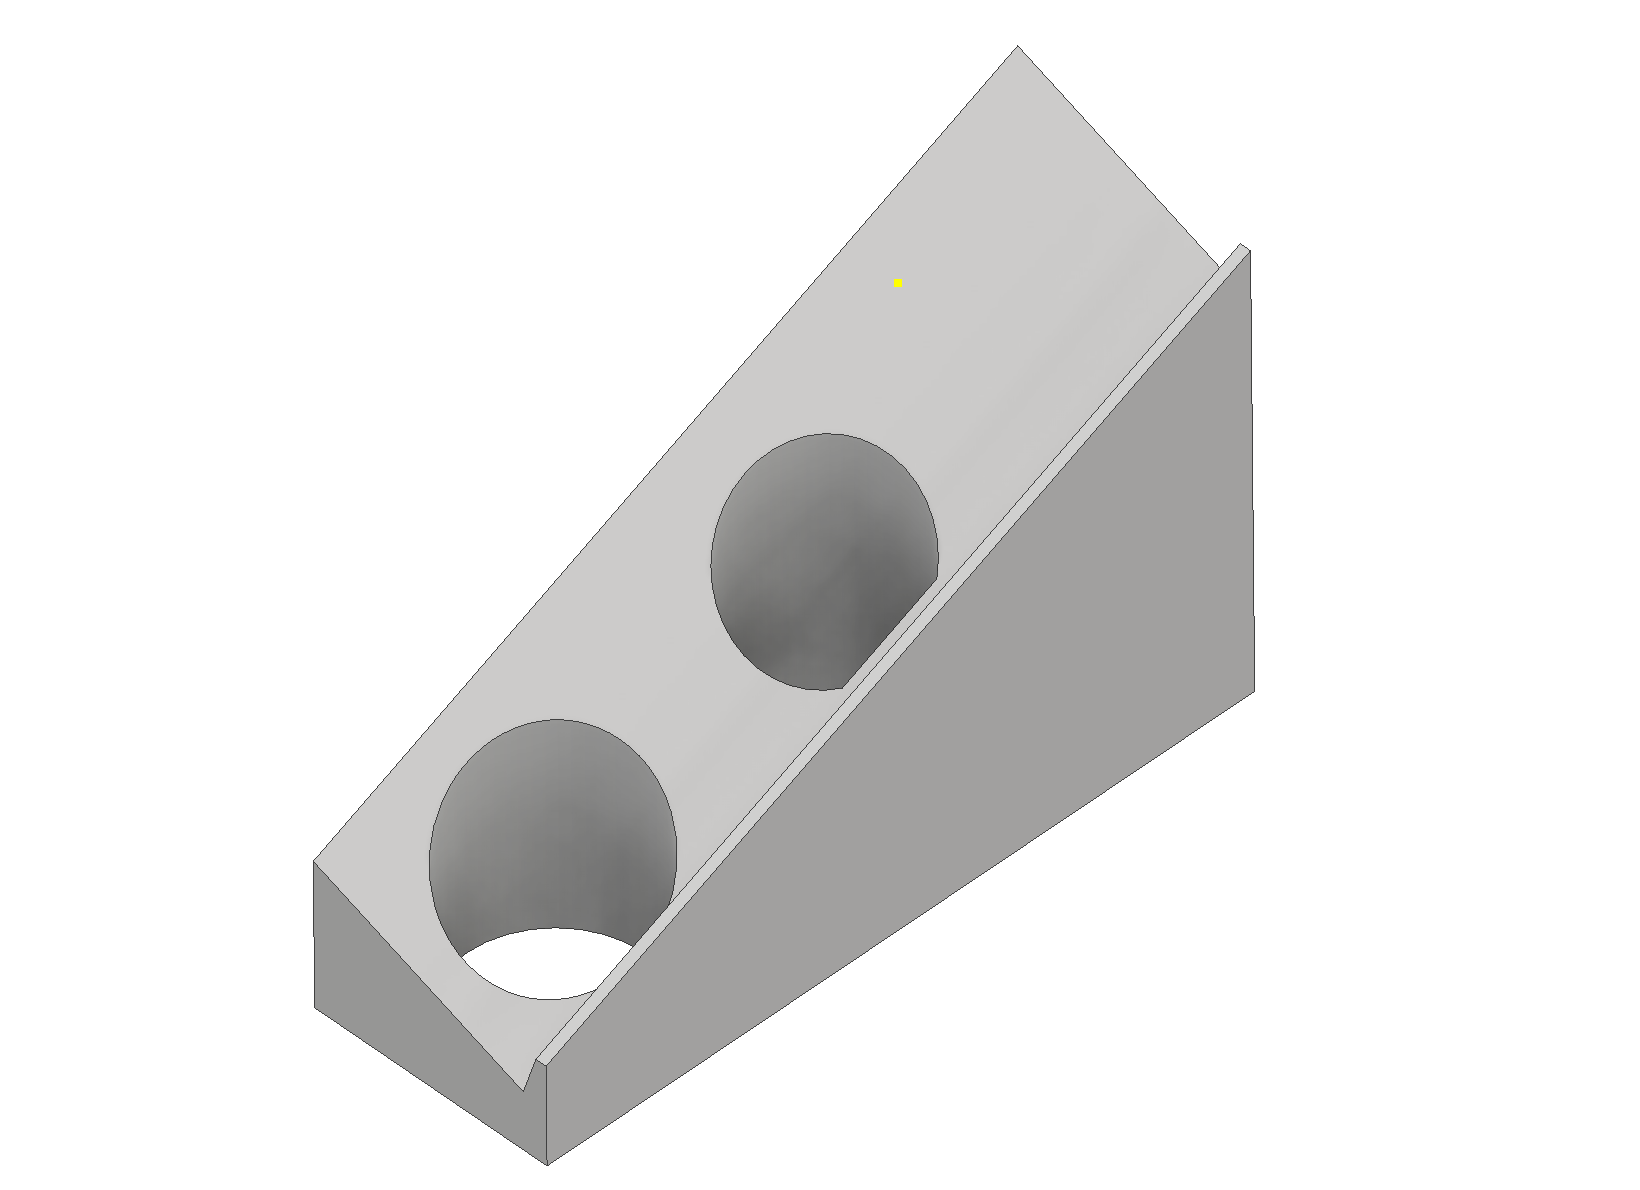
\includegraphics[width=1\linewidth]{HardwareDesign/CoinDispenser/Graphics/sklie.png}
    }
    \caption{Sorterings sklien for mynter}
\end{figure}

Myntene faller ned på en plate med to mindre metallplater der en koblet til en interrupt på PSOC med en pulldown til ground og den andre siden er koblet til VCC.

\begin{figure}[H]
    \centering
    \makebox[\textwidth][c]{%
        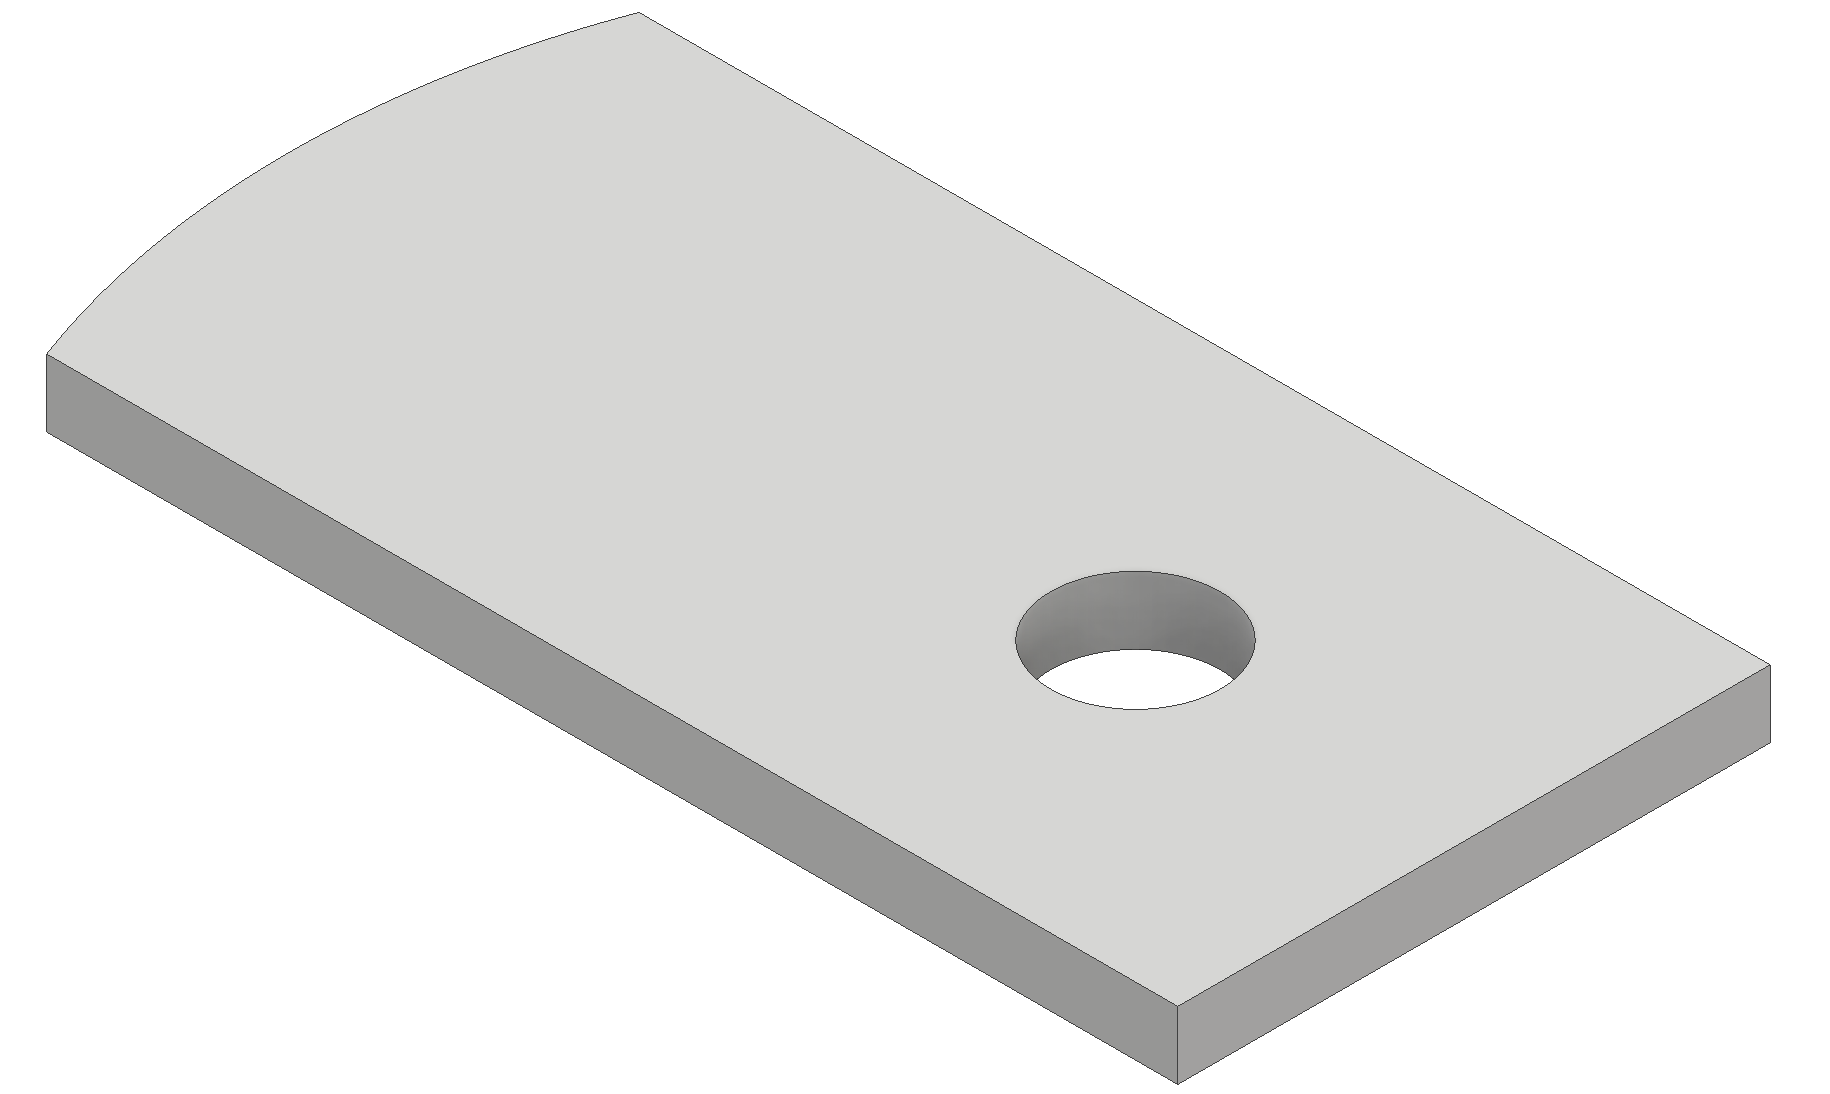
\includegraphics[width=1\linewidth]{HardwareDesign/CoinDispenser/Graphics/stop.png}
    }
    \caption{Platen som mynter lander på}
\end{figure}

Så når mynten lander på platen, skaper den en forbindelse mellom platene, blir mynten samlet eller avvist av en stepper motor ved hjelp av en roterende plate med hull i den.

\begin{figure}[H]
    \centering
    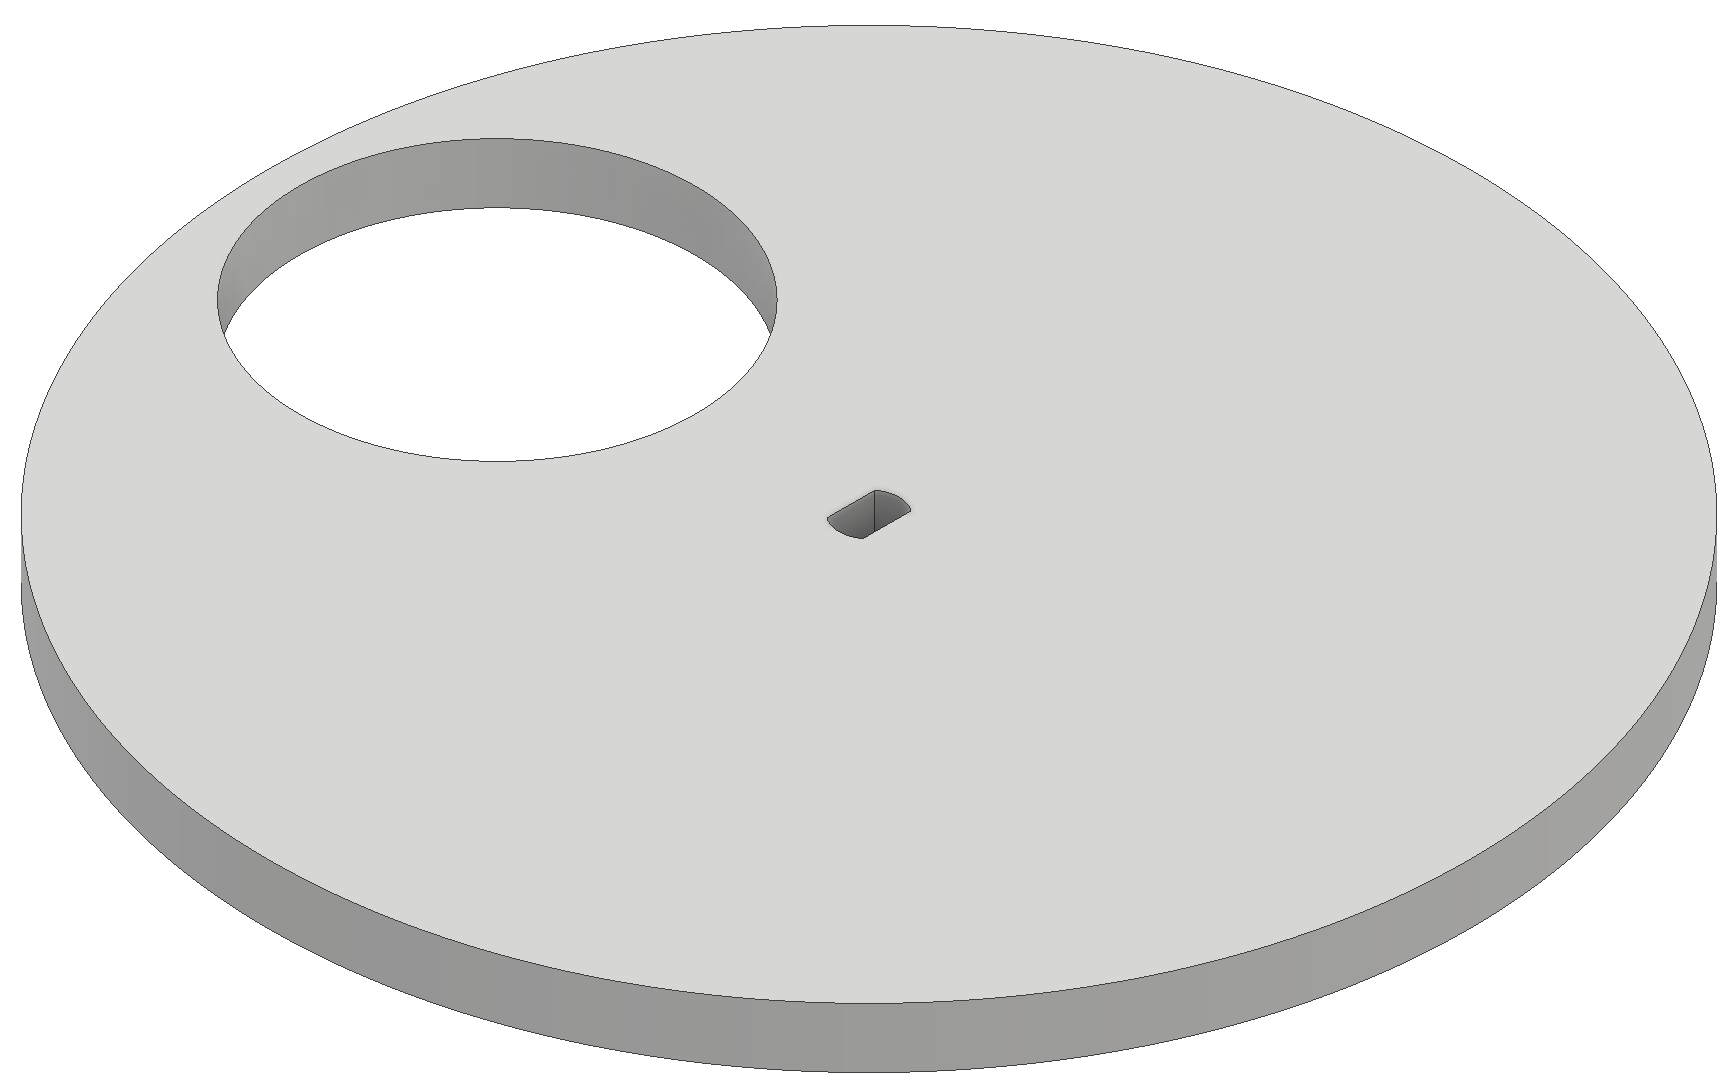
\includegraphics[width=1\linewidth]{HardwareDesign/CoinDispenser/Graphics/disk.png}
    \caption{Sorterings mekanismen som er koblet til en stepper motor}
\end{figure}

Det sammensatte sammensatte systemet er vist under:
\begin{figure}[H]
    \centering
    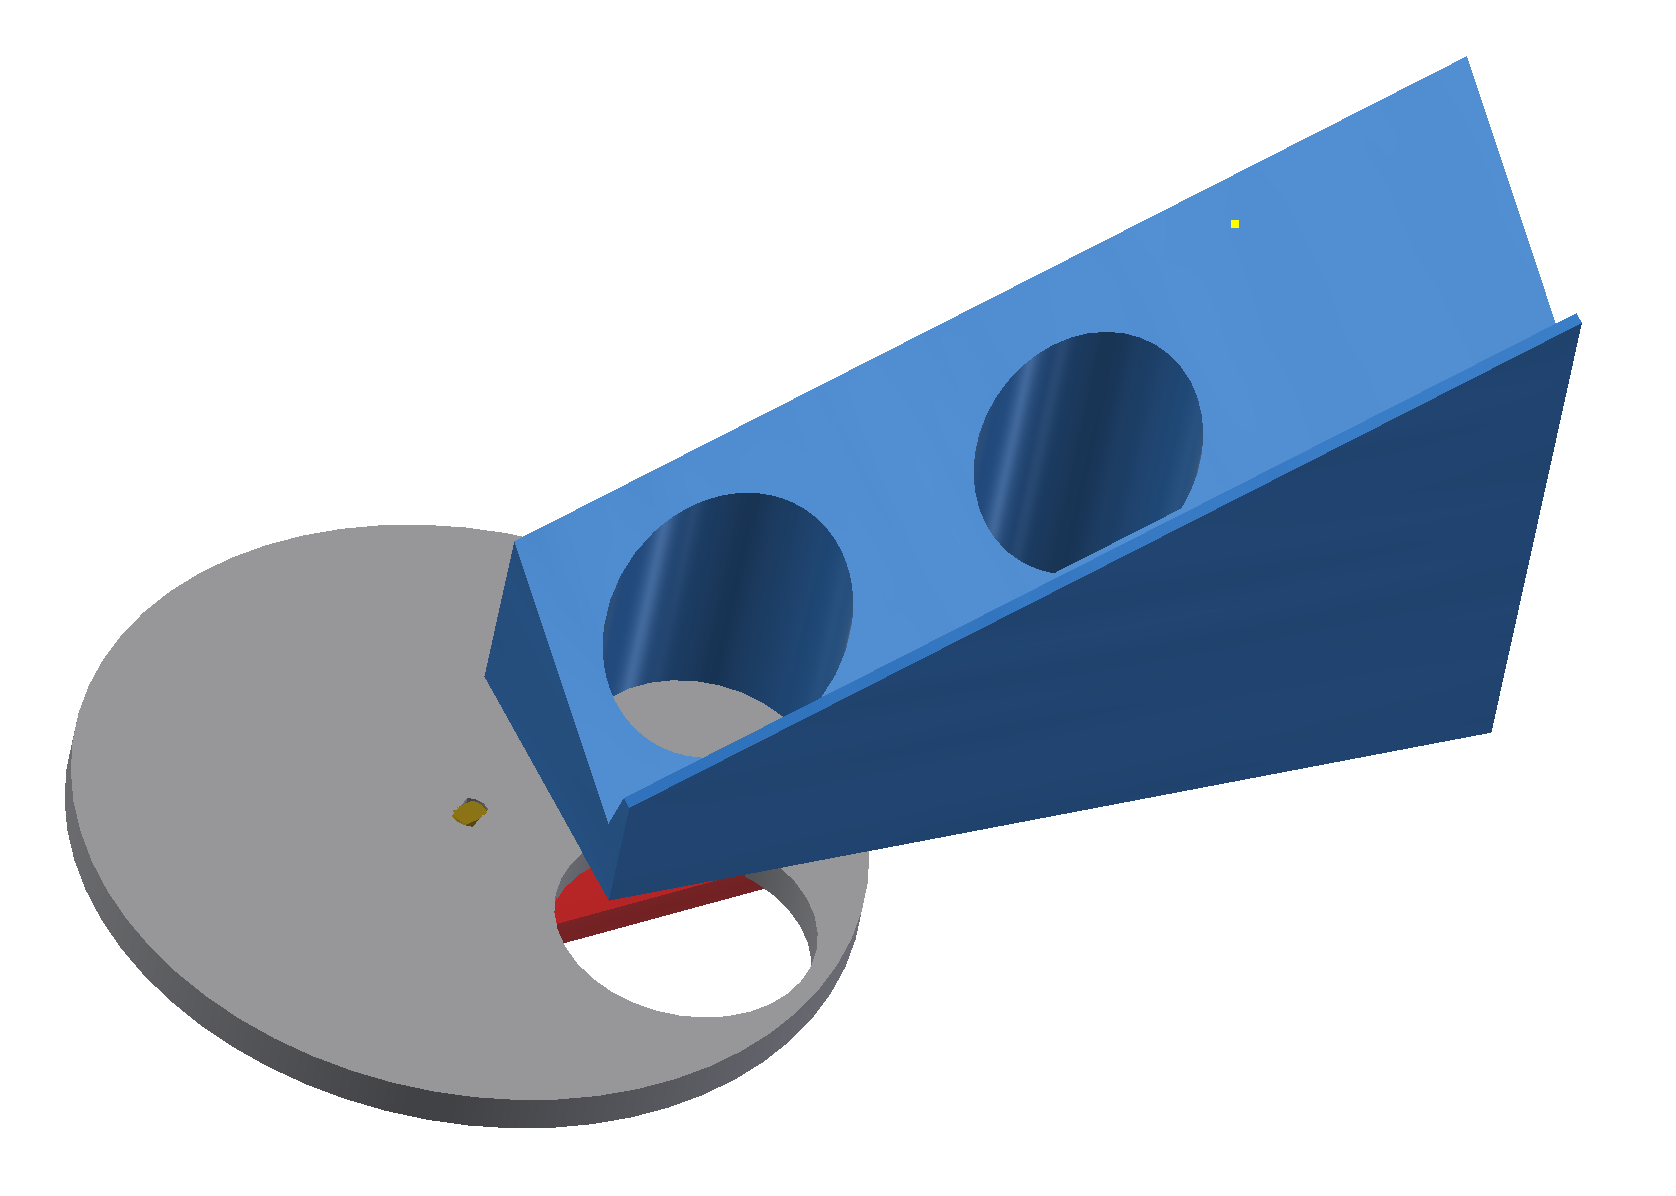
\includegraphics[width=1\linewidth]{Rapport/BallDispenser/CoinDispenser/graphics/coinmaster.png}
    \caption{Den sammensatte CoinDispenser sett ovenfra}
\end{figure}

\begin{figure}[H]
    \centering
    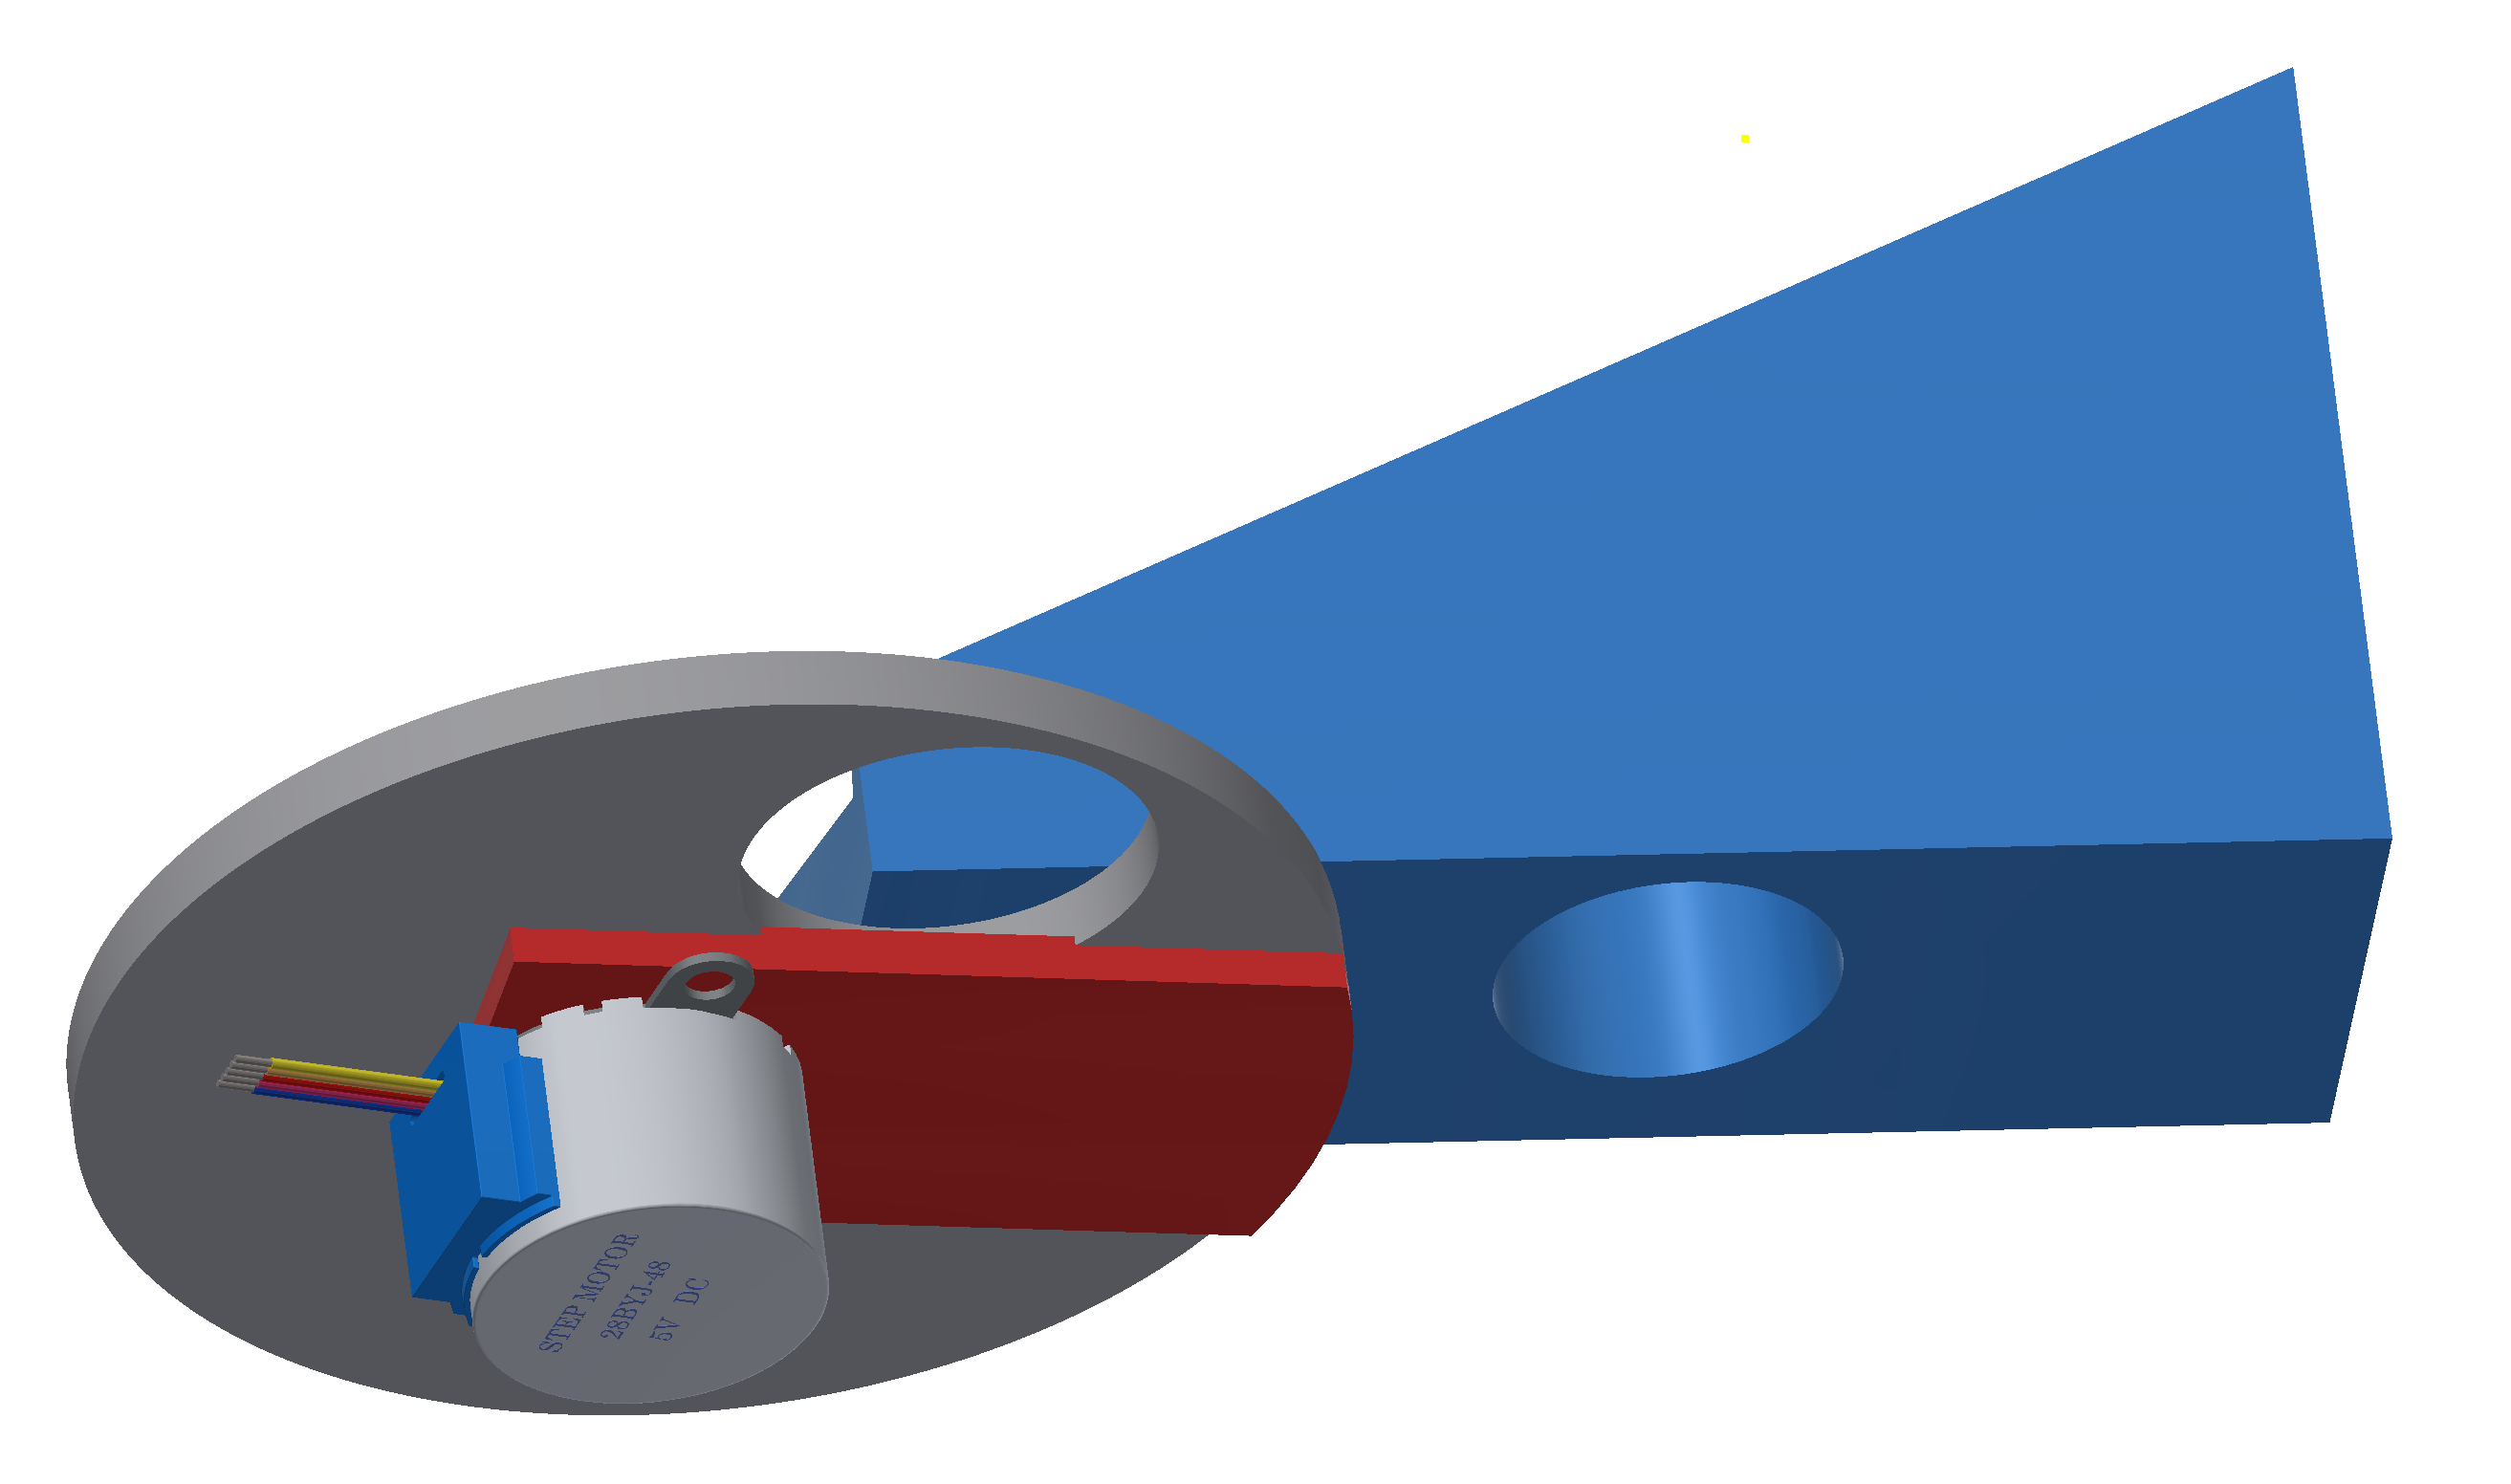
\includegraphics[width=1\linewidth]{Rapport/BallDispenser/CoinDispenser/graphics/coinmaster-under.png}
    \caption{Den sammensatte CoinDispenser sett underfra}
\end{figure}

\subsubsection{Implementering}
Modelene er designet i autodesk inventor. DEt er brukt cura til å konvertere filene fra stl filer til gcode text som brukes til å kontrolere 3D printene på Aarhus Universitet.

\begin{figure}[H]
    \centering
    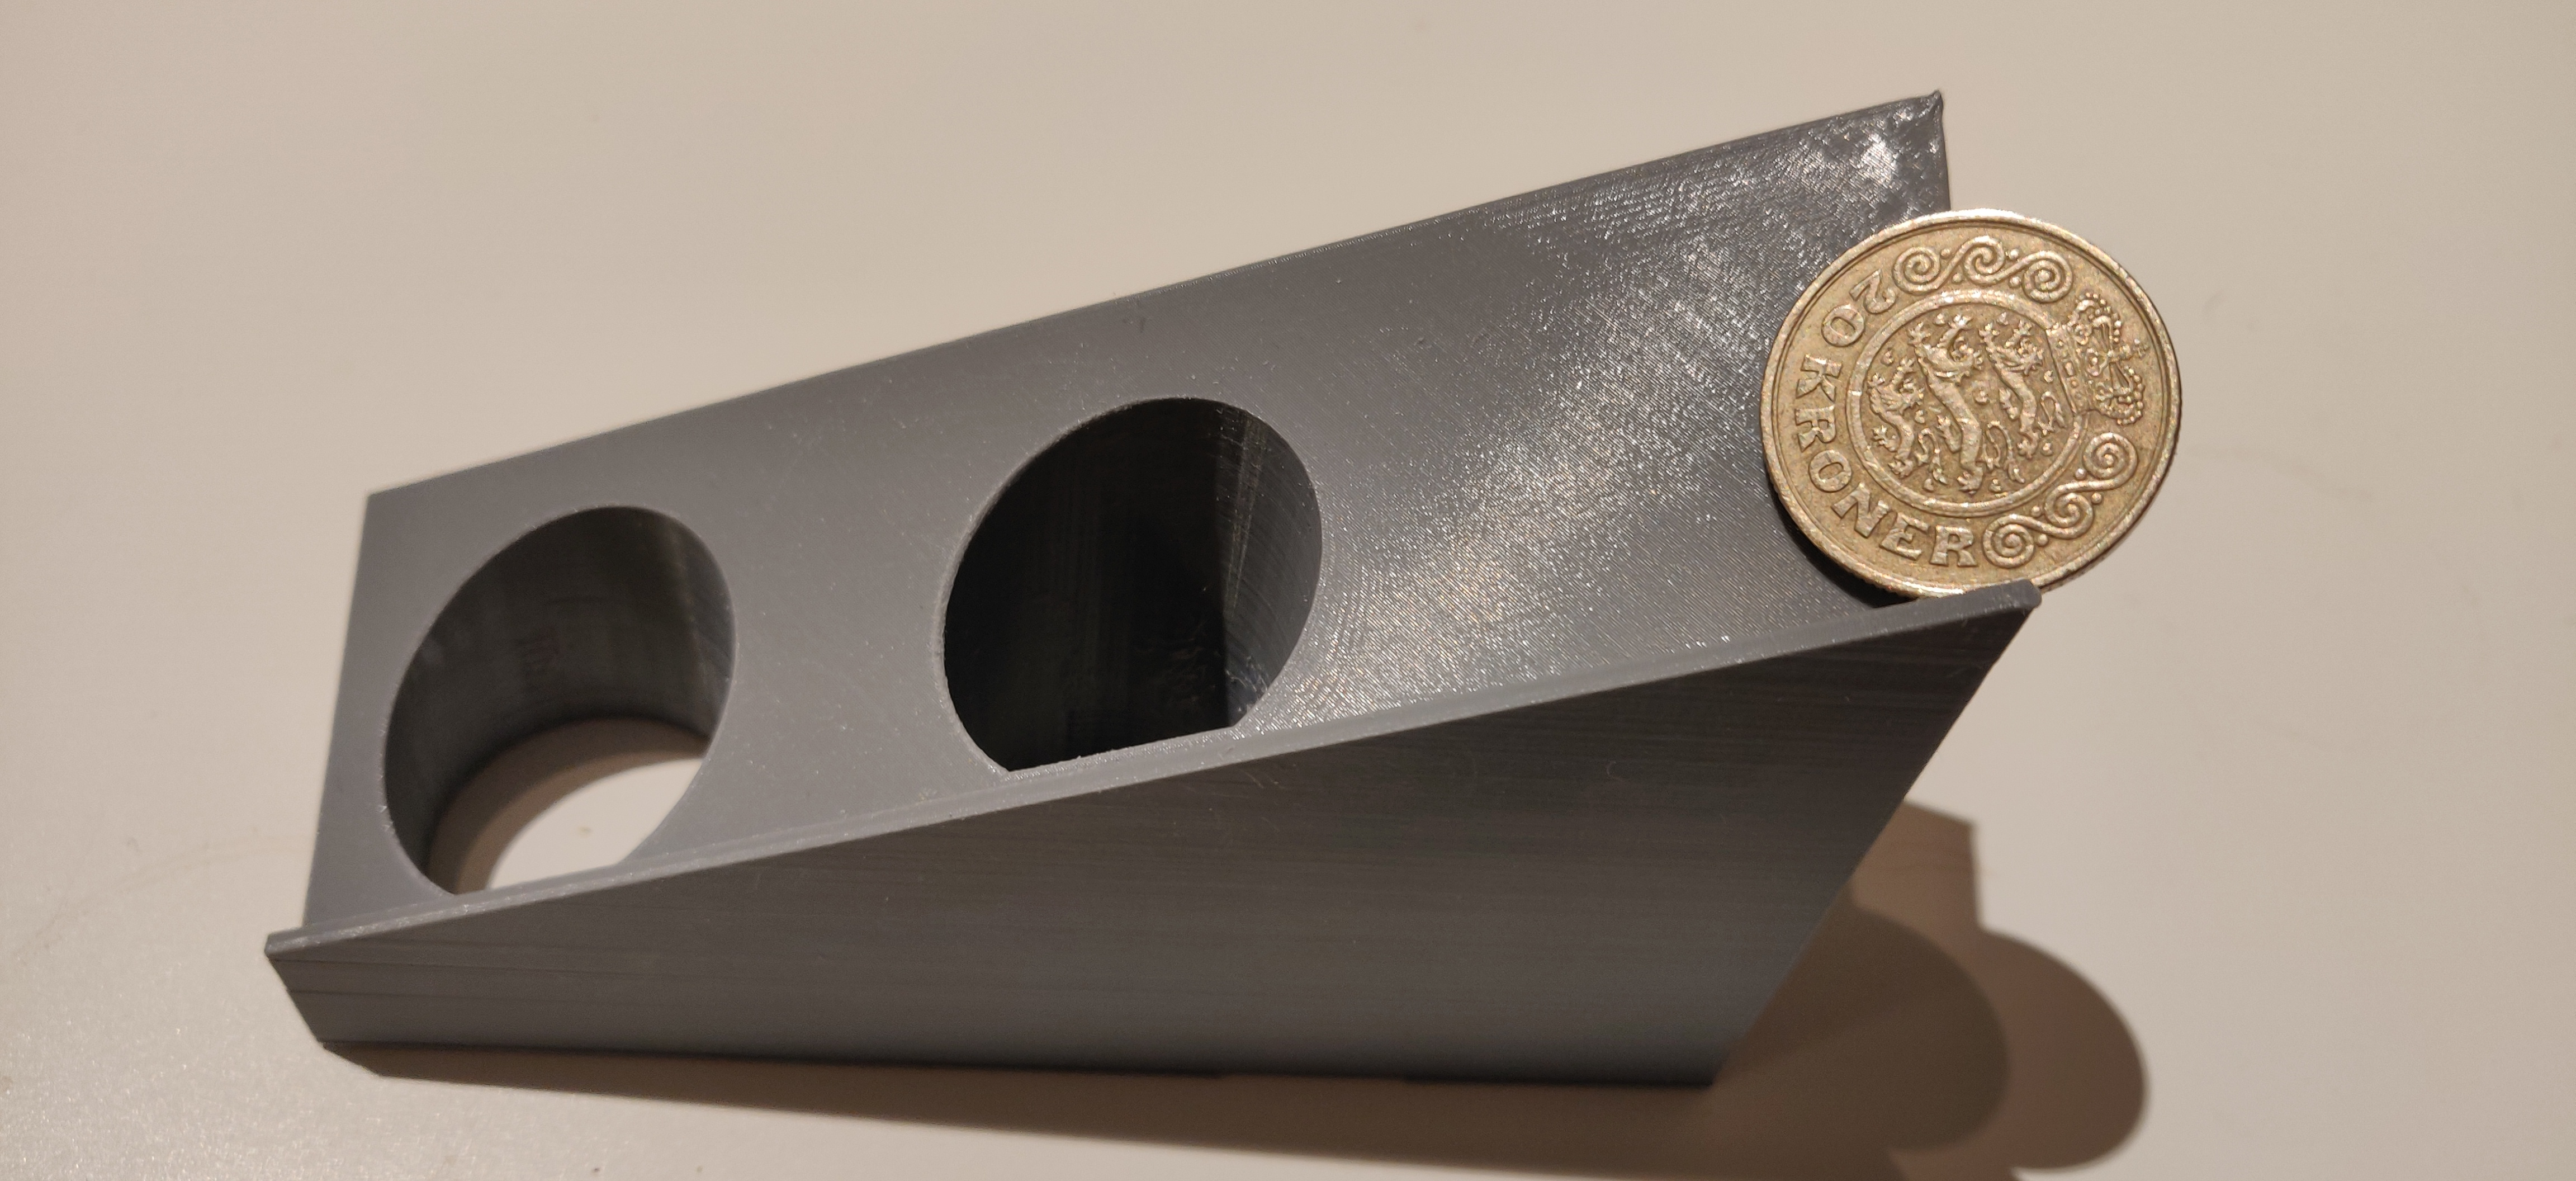
\includegraphics[width=\linewidth]{Modultest/CoinDispenser/CoinHardwareModulTest/Graphic/CoinHardwareTestSetup.jpg}
    \caption{Den printede mynt sorterings sklien}
\end{figure}




\end{document}